\SourceLeaf{198}\begin{center}[2.]\end{center}


[\emph{Satz 1} = Euklid I. 13: Die Winkel, die eine Gerade mit einer andern
bildet, auf der sie steht, sind entweder beide Rechte oder zusammen gleich
zwei Rechten.

\emph{Satz 2} = Euklid I. 5: In jedem gleichschenkligen Dreieck sind die
Winkel an der Grundlinie einander gleich.

\emph{Satz 3} = Euklid I. 6: Sind in einem Dreieck zwei Winkel einander
gleich, so sind auch die den gleichen Winkeln gegenüberliegenden Seiten einander gleich.

\emph{Satz 4}: In einem Dreieck können nicht zwei Winkel gleich Rechten
sein.]

\emph{5. Lehrsatz.} Kein Winkel eines Dreiecks kann dem Nebenwinkel eines
andern Winkels desselben Dreiecks gleich sein.

Es ist nicht möglich, dass $ACB = ABD$.

\textls{Beweis.} Nehmen wir an, es sei $ACB = ABD$ und unterscheiden drei
Fälle.

I. Es sei $AB = AC$. Fig. 1. Also (Satz 2) $ABC = ACB$, folglich
$ABC = ABD$; es sind daher $ABC, ACB$ rechte Winkel [Satz 1], welches
unmöglich ist (Satz 4).



\begin{center}
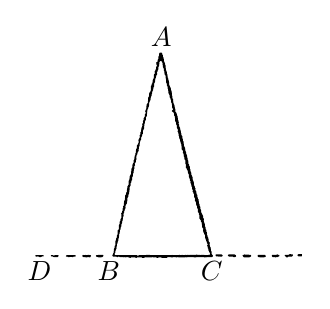
\begin{tikzpicture}[x=0.00477987cm,y=-0.00477987cm]
\fill[even odd rule] (136,623) -- (137,625) -- (141,625) -- (142,626) -- (146,626) -- (147,625) -- (155,626) -- (156,625) -- (161,625) -- (162,624) -- (162,622) -- (161,621) -- (138,621) -- cycle
(96,622) -- (97,624) -- (100,624) -- (104,626) -- (114,626) -- (117,623) -- (116,621) -- (106,621) -- (105,622) -- (103,622) -- (102,621) -- (97,621) -- cycle
(55,622) -- (55,623) -- (57,625) -- (61,624) -- (62,625) -- (65,625) -- (66,626) -- (69,626) -- (73,624) -- (77,624) -- (77,622) -- (76,621) -- (56,621) -- cycle
(646,622) -- (646,624) -- (648,626) -- (651,626) -- (652,627) -- (663,627) -- (664,626) -- (666,626) -- (668,624) -- (666,620) -- (648,620) -- cycle
(216,622) -- (216,623) -- (218,625) -- (222,626) -- (223,627) -- (230,627) -- (231,626) -- (233,626) -- (236,623) -- (236,621) -- (235,620) -- (222,620) -- (221,621) -- (217,621) -- cycle
(180,622) -- (180,624) -- (183,626) -- (188,626) -- (189,627) -- (192,627) -- (193,626) -- (198,626) -- (200,627) -- (203,623) -- (202,621) -- (199,621) -- (198,620) -- (194,620) -- (193,621) -- (190,621) -- (189,620) -- (187,621) -- (184,621) -- (182,620) -- cycle
(704,621) -- (703,620) -- (700,620) -- (699,619) -- (697,619) -- (696,620) -- (685,620) -- (684,621) -- (684,624) -- (686,626) -- (692,626) -- (694,627) -- (695,626) -- (699,626) -- (700,625) -- (702,625) -- (704,623) -- cycle
(606,621) -- (607,624) -- (610,627) -- (623,627) -- (629,624) -- (629,622) -- (627,620) -- (611,619) -- (610,620) -- (607,620) -- cycle
(567,621) -- (567,622) -- (570,625) -- (581,625) -- (582,626) -- (586,626) -- (589,624) -- (588,621) -- (585,619) -- (569,619) -- cycle
(534,620) -- (534,622) -- (536,624) -- (541,624) -- (542,625) -- (544,625) -- (545,624) -- (547,625) -- (551,625) -- (553,622) -- (553,621) -- (550,619) -- (535,619) -- cycle
(752,620) -- (752,621) -- (755,624) -- (763,624) -- (764,623) -- (764,619) -- (763,618) -- (755,618) -- cycle
(740,620) -- (739,619) -- (735,619) -- (734,618) -- (732,618) -- (728,620) -- (719,620) -- (718,622) -- (723,627) -- (725,627) -- (727,625) -- (736,625) -- (739,623) -- cycle
(386,82) -- (384,86) -- (384,90) -- (382,94) -- (382,99) -- (380,102) -- (380,106) -- (376,109) -- (377,111) -- (377,114) -- (378,115) -- (378,118) -- (376,121) -- (376,125) -- (375,126) -- (375,128) -- (372,133) -- (373,137) -- (370,141) -- (370,149) -- (367,156) -- (367,161) -- (366,162) -- (366,164) -- (364,166) -- (364,169) -- (362,171) -- (362,183) -- (361,184) -- (361,186) -- (358,189) -- (357,199) -- (355,202) -- (355,210) -- (354,211) -- (354,216) -- (351,220) -- (351,223) -- (350,224) -- (350,231) -- (347,238) -- (348,240) -- (348,244) -- (346,246) -- (346,252) -- (343,257) -- (343,261) -- (341,265) -- (342,269) -- (339,272) -- (340,276) -- (337,283) -- (336,292) -- (334,294) -- (334,300) -- (332,302) -- (333,307) -- (329,315) -- (330,321) -- (327,327) -- (325,329) -- (325,336) -- (323,339) -- (323,342) -- (322,343) -- (322,349) -- (321,350) -- (321,353) -- (319,357) -- (318,366) -- (316,369) -- (316,375) -- (314,377) -- (314,379) -- (313,380) -- (313,387) -- (310,392) -- (310,398) -- (309,399) -- (310,403) -- (306,411) -- (305,420) -- (303,424) -- (303,433) -- (300,438) -- (299,446) -- (298,447) -- (298,453) -- (296,455) -- (296,459) -- (294,462) -- (293,474) -- (291,477) -- (290,489) -- (288,491) -- (289,494) -- (287,497) -- (287,503) -- (286,504) -- (285,508) -- (283,510) -- (284,512) -- (284,521) -- (281,526) -- (281,530) -- (279,532) -- (279,538) -- (277,542) -- (277,552) -- (274,555) -- (274,565) -- (272,568) -- (272,573) -- (270,576) -- (269,582) -- (268,583) -- (268,594) -- (266,596) -- (266,600) -- (264,604) -- (263,615) -- (262,616) -- (262,618) -- (260,620) -- (260,623) -- (263,625) -- (271,625) -- (272,626) -- (274,626) -- (275,625) -- (278,625) -- (279,626) -- (289,626) -- (290,627) -- (292,626) -- (294,626) -- (295,627) -- (297,626) -- (301,626) -- (302,627) -- (305,627) -- (306,628) -- (308,628) -- (309,627) -- (321,627) -- (322,628) -- (324,628) -- (325,627) -- (338,627) -- (339,628) -- (344,628) -- (347,626) -- (349,627) -- (365,627) -- (366,626) -- (368,626) -- (369,627) -- (373,627) -- (375,626) -- (379,628) -- (381,628) -- (382,627) -- (390,627) -- (391,628) -- (404,628) -- (407,626) -- (415,626) -- (416,627) -- (420,627) -- (421,626) -- (428,626) -- (429,627) -- (431,627) -- (432,626) -- (435,626) -- (436,627) -- (453,627) -- (454,626) -- (456,626) -- (457,627) -- (459,626) -- (476,626) -- (477,627) -- (482,627) -- (483,626) -- (503,626) -- (505,627) -- (507,626) -- (509,627) -- (510,626) -- (525,626) -- (527,624) -- (527,622) -- (524,618) -- (524,613) -- (522,609) -- (522,604) -- (521,603) -- (521,600) -- (519,598) -- (519,595) -- (518,594) -- (519,588) -- (516,584) -- (515,575) -- (513,572) -- (513,569) -- (511,567) -- (512,564) -- (511,563) -- (511,560) -- (510,559) -- (510,554) -- (508,552) -- (508,548) -- (506,544) -- (506,539) -- (505,538) -- (505,535) -- (503,533) -- (503,530) -- (502,529) -- (503,527) -- (503,524) -- (501,522) -- (501,517) -- (496,507) -- (496,502) -- (494,498) -- (494,493) -- (492,490) -- (492,487) -- (490,483) -- (489,473) -- (487,471) -- (487,468) -- (486,467) -- (486,461) -- (484,459) -- (484,457) -- (483,456) -- (483,452) -- (480,447) -- (481,444) -- (479,441) -- (479,439) -- (477,435) -- (476,426) -- (473,419) -- (473,413) -- (471,411) -- (471,409) -- (470,408) -- (470,404) -- (469,403) -- (469,400) -- (468,399) -- (468,397) -- (467,396) -- (467,392) -- (466,391) -- (466,386) -- (464,383) -- (464,380) -- (462,378) -- (462,372) -- (461,371) -- (461,368) -- (460,367) -- (460,363) -- (459,362) -- (458,355) -- (456,351) -- (456,348) -- (454,344) -- (453,336) -- (450,330) -- (449,319) -- (447,316) -- (447,312) -- (446,311) -- (446,305) -- (443,301) -- (443,297) -- (442,296) -- (442,292) -- (441,291) -- (441,288) -- (440,287) -- (440,283) -- (437,277) -- (437,273) -- (436,272) -- (436,269) -- (437,267) -- (435,265) -- (435,262) -- (434,261) -- (434,256) -- (433,255) -- (433,251) -- (432,250) -- (430,242) -- (427,239) -- (427,232) -- (426,231) -- (426,228) -- (425,227) -- (425,223) -- (422,216) -- (421,206) -- (419,203) -- (419,197) -- (418,196) -- (418,189) -- (417,188) -- (417,184) -- (415,181) -- (415,177) -- (411,168) -- (411,161) -- (410,160) -- (410,157) -- (409,156) -- (408,150) -- (407,149) -- (407,144) -- (406,143) -- (406,140) -- (405,139) -- (405,135) -- (402,128) -- (401,116) -- (400,115) -- (400,112) -- (397,105) -- (396,96) -- (394,93) -- (394,89) -- (393,88) -- (392,84) -- (390,82) -- cycle
(388,104) -- (390,104) -- (391,105) -- (391,107) -- (393,109) -- (393,111) -- (394,112) -- (393,115) -- (394,116) -- (394,120) -- (397,126) -- (397,131) -- (398,132) -- (398,137) -- (399,138) -- (399,141) -- (401,143) -- (402,153) -- (403,154) -- (403,162) -- (405,166) -- (405,170) -- (407,173) -- (407,178) -- (408,179) -- (408,183) -- (409,184) -- (409,190) -- (412,196) -- (412,201) -- (414,203) -- (414,205) -- (416,209) -- (416,214) -- (418,218) -- (419,229) -- (421,232) -- (421,234) -- (418,237) -- (418,238) -- (423,242) -- (423,244) -- (424,245) -- (424,249) -- (426,252) -- (427,265) -- (429,268) -- (429,272) -- (431,276) -- (431,281) -- (434,287) -- (434,290) -- (433,292) -- (435,295) -- (435,298) -- (436,299) -- (436,303) -- (437,304) -- (438,311) -- (440,314) -- (440,318) -- (441,319) -- (441,322) -- (443,326) -- (443,330) -- (444,331) -- (444,339) -- (448,344) -- (447,349) -- (449,351) -- (449,355) -- (450,356) -- (450,359) -- (451,360) -- (451,365) -- (454,369) -- (454,378) -- (456,381) -- (455,383) -- (455,388) -- (458,391) -- (458,393) -- (460,396) -- (461,402) -- (463,406) -- (463,412) -- (466,419) -- (466,422) -- (468,425) -- (467,429) -- (469,431) -- (469,433) -- (470,434) -- (470,438) -- (472,440) -- (472,445) -- (474,448) -- (473,452) -- (475,454) -- (475,456) -- (477,459) -- (477,466) -- (480,471) -- (479,475) -- (482,480) -- (483,488) -- (485,491) -- (485,495) -- (487,498) -- (487,506) -- (490,509) -- (490,513) -- (491,514) -- (491,523) -- (495,528) -- (495,531) -- (497,533) -- (499,548) -- (502,551) -- (501,553) -- (501,557) -- (502,558) -- (502,560) -- (504,562) -- (504,565) -- (506,567) -- (507,578) -- (509,580) -- (509,583) -- (511,585) -- (511,588) -- (513,591) -- (513,594) -- (512,595) -- (512,597) -- (514,599) -- (513,602) -- (515,604) -- (515,607) -- (520,617) -- (520,618) -- (518,620) -- (515,620) -- (514,621) -- (505,621) -- (504,620) -- (495,620) -- (493,621) -- (492,620) -- (486,620) -- (484,619) -- (483,620) -- (465,620) -- (464,621) -- (462,620) -- (458,620) -- (457,621) -- (455,620) -- (453,620) -- (452,621) -- (447,621) -- (446,620) -- (444,620) -- (443,621) -- (440,621) -- (439,620) -- (437,620) -- (436,621) -- (420,621) -- (419,620) -- (417,621) -- (360,621) -- (359,620) -- (350,620) -- (349,621) -- (330,621) -- (329,622) -- (326,622) -- (325,621) -- (268,621) -- (266,619) -- (266,616) -- (268,613) -- (268,609) -- (269,608) -- (269,606) -- (271,604) -- (270,601) -- (271,600) -- (271,597) -- (272,596) -- (272,591) -- (274,588) -- (274,585) -- (276,581) -- (276,576) -- (277,575) -- (278,564) -- (279,563) -- (279,560) -- (280,559) -- (280,554) -- (282,551) -- (282,547) -- (284,543) -- (284,538) -- (286,534) -- (286,530) -- (287,529) -- (288,520) -- (290,516) -- (289,512) -- (290,511) -- (290,509) -- (291,508) -- (291,504) -- (292,503) -- (292,501) -- (294,498) -- (294,495) -- (295,494) -- (294,490) -- (296,488) -- (296,486) -- (298,484) -- (298,481) -- (299,480) -- (300,468) -- (302,465) -- (302,461) -- (303,460) -- (303,458) -- (304,457) -- (304,453) -- (305,452) -- (306,439) -- (308,436) -- (308,429) -- (310,427) -- (310,423) -- (312,421) -- (312,414) -- (314,411) -- (314,405) -- (316,402) -- (317,392) -- (318,391) -- (318,384) -- (320,382) -- (319,378) -- (322,373) -- (322,369) -- (324,365) -- (323,359) -- (324,358) -- (324,355) -- (326,353) -- (327,347) -- (329,345) -- (329,343) -- (330,342) -- (329,340) -- (330,338) -- (330,333) -- (332,331) -- (332,324) -- (333,323) -- (333,319) -- (334,318) -- (334,316) -- (336,314) -- (336,309) -- (339,303) -- (339,300) -- (341,298) -- (341,290) -- (344,284) -- (345,271) -- (346,270) -- (346,266) -- (349,260) -- (349,254) -- (351,252) -- (353,234) -- (355,231) -- (355,229) -- (357,225) -- (358,214) -- (361,208) -- (362,200) -- (364,197) -- (364,193) -- (365,192) -- (366,185) -- (368,182) -- (369,175) -- (371,172) -- (371,164) -- (373,160) -- (374,151) -- (375,150) -- (377,142) -- (379,140) -- (379,137) -- (378,135) -- (380,132) -- (380,130) -- (382,126) -- (382,121) -- (384,117) -- (385,107) -- cycle;
\node[inner sep=0pt] at (390,41) {$A$};
\node[inner sep=0pt] at (66,662) {$D$};
\node[inner sep=0pt] at (250,662) {$B$};
\node[inner sep=0pt] at (524,663) {$C$};
\end{tikzpicture}
\\[3pt]Fig. 1.
\end{center}

II. Es sei $AB$ kleiner als $AC$. (Fig. 2.) Es liegt daher $B$ innerhalb
einer Kugelfläche, deren Mittelpunkt $A$, Halbmesser $=AC$. Die gerade Linie
$CB$ über $B$ hinaus verlängert muss folglich die Kugelfläche schneiden; das
geschehe in $E$. Es ist also $AE=AC$, daher $AEB=ACB$ (Satz 2), dann
$AEB=ABD=ABE$, ferner (Satz 3) $AB=AE=AC$ gegen die Voraussetzung.



\begin{center}
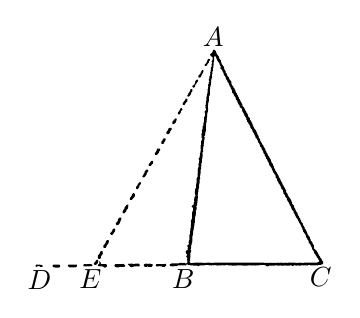
\begin{tikzpicture}[x=0.00500000cm,y=-0.00500000cm]
\fill[even odd rule] (110,613) -- (110,615) -- (114,618) -- (129,618) -- (133,616) -- (133,612) -- (132,611) -- (112,611) -- cycle
(71,613) -- (71,615) -- (74,618) -- (77,618) -- (78,619) -- (87,619) -- (90,617) -- (90,613) -- (88,611) -- (74,611) -- cycle
(28,613) -- (28,615) -- (30,617) -- (34,615) -- (38,615) -- (40,617) -- (45,617) -- (46,616) -- (46,614) -- (44,612) -- (40,612) -- (39,611) -- (30,611) -- cycle
(149,612) -- (149,614) -- (151,616) -- (159,616) -- (160,615) -- (164,616) -- (165,615) -- (171,615) -- (172,614) -- (172,612) -- (169,610) -- (158,610) -- (157,611) -- (155,610) -- (152,610) -- cycle
(359,611) -- (357,609) -- (355,610) -- (335,610) -- (333,612) -- (333,614) -- (335,616) -- (340,616) -- (341,615) -- (344,615) -- (345,616) -- (349,616) -- (350,617) -- (355,617) -- (359,614) -- cycle
(303,611) -- (303,615) -- (306,617) -- (310,617) -- (311,616) -- (313,616) -- (314,617) -- (322,617) -- (325,614) -- (325,611) -- (324,610) -- (320,610) -- (319,609) -- (317,609) -- (316,610) -- (314,609) -- (312,610) -- (310,609) -- (307,609) -- cycle
(263,610) -- (263,611) -- (269,617) -- (271,618) -- (273,617) -- (276,617) -- (277,616) -- (283,616) -- (284,615) -- (286,615) -- (287,616) -- (291,616) -- (292,615) -- (292,611) -- (290,609) -- (280,609) -- (279,610) -- (276,610) -- (275,609) -- (269,609) -- (267,610) -- (266,609) -- (264,609) -- cycle
(255,613) -- (251,609) -- (249,610) -- (231,610) -- (229,612) -- (228,615) -- (230,617) -- (232,617) -- (233,618) -- (240,618) -- (241,617) -- (253,617) -- (255,615) -- cycle
(186,612) -- (186,614) -- (187,615) -- (190,615) -- (191,616) -- (199,616) -- (203,619) -- (205,619) -- (209,616) -- (209,612) -- (207,610) -- (195,610) -- (193,608) -- (193,605) -- (191,603) -- (189,604) -- (190,606) -- (190,609) -- cycle
(186,599) -- (183,599) -- (176,608) -- (176,610) -- (178,612) -- (181,612) -- (186,607) -- (186,605) -- (187,604) -- (187,600) -- cycle
(197,577) -- (194,577) -- (192,579) -- (190,584) -- (186,588) -- (186,594) -- (188,597) -- (191,597) -- (193,595) -- (194,593) -- (194,590) -- (199,583) -- (198,581) -- (198,578) -- cycle
(212,549) -- (209,549) -- (208,550) -- (208,551) -- (206,553) -- (206,556) -- (200,563) -- (200,567) -- (202,569) -- (205,569) -- (207,567) -- (209,562) -- (213,557) -- (214,551) -- cycle
(229,520) -- (226,520) -- (223,523) -- (223,525) -- (221,527) -- (221,528) -- (217,532) -- (217,533) -- (220,536) -- (223,536) -- (230,526) -- (230,521) -- cycle
(245,492) -- (241,492) -- (238,495) -- (237,497) -- (237,500) -- (232,506) -- (232,509) -- (234,511) -- (237,511) -- (241,507) -- (246,495) -- (246,493) -- cycle
(263,459) -- (260,459) -- (254,466) -- (254,468) -- (249,476) -- (249,479) -- (251,481) -- (253,481) -- (258,476) -- (259,472) -- (262,469) -- (262,467) -- (263,466) -- (263,462) -- (264,461) -- cycle
(278,430) -- (276,430) -- (273,433) -- (271,438) -- (269,440) -- (267,444) -- (267,446) -- (268,447) -- (272,447) -- (280,438) -- (280,433) -- cycle
(294,402) -- (292,402) -- (288,406) -- (286,411) -- (284,413) -- (283,415) -- (283,418) -- (285,420) -- (287,420) -- (291,414) -- (292,410) -- (295,407) -- (295,403) -- cycle
(312,370) -- (310,370) -- (305,375) -- (305,378) -- (302,381) -- (302,383) -- (299,387) -- (299,388) -- (301,390) -- (305,389) -- (310,382) -- (310,380) -- (314,373) -- (314,372) -- cycle
(325,348) -- (322,348) -- (315,357) -- (315,359) -- (317,361) -- (320,361) -- (326,354) -- (326,349) -- cycle
(343,317) -- (337,317) -- (336,318) -- (336,320) -- (333,326) -- (331,328) -- (331,332) -- (332,333) -- (336,333) -- (341,327) -- (341,325) -- (344,322) -- (344,318) -- cycle
(357,291) -- (353,291) -- (351,293) -- (350,296) -- (347,299) -- (347,304) -- (348,305) -- (352,305) -- (354,303) -- (354,301) -- (356,299) -- (358,295) -- (358,292) -- cycle
(372,264) -- (367,264) -- (366,265) -- (364,270) -- (360,275) -- (360,278) -- (362,280) -- (366,280) -- (369,276) -- (370,272) -- (373,269) -- (373,265) -- cycle
(385,240) -- (383,240) -- (375,249) -- (375,253) -- (377,255) -- (381,253) -- (384,250) -- (385,246) -- (386,245) -- (386,241) -- cycle
(399,214) -- (397,214) -- (395,216) -- (394,219) -- (389,226) -- (389,229) -- (390,230) -- (393,230) -- (395,228) -- (397,224) -- (397,222) -- (401,218) -- cycle
(412,190) -- (409,190) -- (408,191) -- (408,193) -- (402,201) -- (401,204) -- (403,206) -- (406,206) -- (409,201) -- (413,197) -- (413,191) -- cycle
(425,166) -- (422,166) -- (421,167) -- (421,169) -- (419,171) -- (419,173) -- (416,176) -- (416,178) -- (413,182) -- (413,183) -- (415,185) -- (417,185) -- (423,178) -- (423,175) -- (426,171) -- (426,167) -- cycle
(439,142) -- (437,142) -- (434,145) -- (433,147) -- (433,150) -- (431,154) -- (426,158) -- (426,160) -- (428,162) -- (430,162) -- (433,159) -- (433,156) -- (440,146) -- (440,143) -- cycle
(453,117) -- (452,117) -- (449,120) -- (446,127) -- (441,132) -- (441,135) -- (443,137) -- (445,137) -- (448,134) -- (448,132) -- (450,130) -- (450,128) -- (452,126) -- (454,122) -- (454,118) -- cycle
(469,89) -- (467,89) -- (464,92) -- (464,94) -- (461,100) -- (457,104) -- (457,106) -- (458,107) -- (461,107) -- (464,104) -- (464,102) -- (468,98) -- (468,95) -- (470,93) -- (470,90) -- cycle
(480,66) -- (478,68) -- (477,72) -- (471,78) -- (472,81) -- (477,85) -- (477,92) -- (475,95) -- (475,97) -- (476,98) -- (476,100) -- (475,101) -- (475,109) -- (473,111) -- (473,118) -- (472,119) -- (472,122) -- (471,123) -- (472,128) -- (471,129) -- (471,132) -- (469,134) -- (469,139) -- (468,140) -- (468,144) -- (469,145) -- (469,147) -- (467,149) -- (468,151) -- (466,155) -- (466,158) -- (467,160) -- (466,161) -- (466,164) -- (465,165) -- (464,178) -- (463,179) -- (463,183) -- (462,184) -- (462,187) -- (461,188) -- (462,194) -- (461,195) -- (461,198) -- (460,199) -- (460,205) -- (459,206) -- (459,208) -- (460,209) -- (459,213) -- (460,214) -- (460,217) -- (461,219) -- (457,223) -- (457,225) -- (458,226) -- (458,233) -- (456,237) -- (456,246) -- (455,247) -- (455,251) -- (454,252) -- (454,259) -- (452,261) -- (452,268) -- (450,270) -- (451,276) -- (449,280) -- (449,283) -- (450,284) -- (449,289) -- (451,291) -- (451,293) -- (450,294) -- (450,296) -- (448,298) -- (448,308) -- (447,309) -- (447,317) -- (448,319) -- (447,320) -- (447,324) -- (446,325) -- (446,328) -- (445,329) -- (446,334) -- (444,336) -- (444,340) -- (442,342) -- (442,344) -- (444,346) -- (444,347) -- (443,348) -- (443,353) -- (441,356) -- (441,358) -- (442,359) -- (442,364) -- (440,366) -- (440,371) -- (439,372) -- (439,374) -- (440,375) -- (440,378) -- (439,379) -- (439,389) -- (437,392) -- (437,403) -- (436,404) -- (435,417) -- (433,419) -- (433,424) -- (432,425) -- (432,432) -- (433,433) -- (434,437) -- (431,440) -- (431,445) -- (430,446) -- (431,451) -- (430,452) -- (430,456) -- (429,457) -- (429,459) -- (424,463) -- (424,464) -- (428,468) -- (428,472) -- (427,473) -- (427,476) -- (425,478) -- (426,480) -- (425,482) -- (425,494) -- (422,501) -- (422,504) -- (423,505) -- (423,507) -- (422,508) -- (422,518) -- (421,519) -- (421,525) -- (420,526) -- (420,533) -- (418,537) -- (418,541) -- (419,542) -- (418,545) -- (419,547) -- (417,550) -- (417,554) -- (416,555) -- (417,557) -- (417,560) -- (413,563) -- (413,565) -- (415,568) -- (414,570) -- (414,572) -- (415,573) -- (413,575) -- (411,575) -- (409,577) -- (410,583) -- (413,586) -- (413,587) -- (410,590) -- (413,595) -- (413,597) -- (412,598) -- (413,600) -- (413,606) -- (411,608) -- (407,608) -- (406,607) -- (403,607) -- (402,608) -- (400,607) -- (393,607) -- (392,608) -- (374,608) -- (368,611) -- (369,614) -- (370,615) -- (378,616) -- (379,615) -- (387,615) -- (389,613) -- (398,613) -- (399,612) -- (401,613) -- (409,613) -- (412,610) -- (413,610) -- (415,612) -- (419,612) -- (420,613) -- (427,613) -- (428,614) -- (439,614) -- (440,615) -- (442,615) -- (445,613) -- (457,613) -- (458,612) -- (467,612) -- (468,613) -- (475,613) -- (476,612) -- (478,613) -- (481,613) -- (482,612) -- (484,612) -- (485,613) -- (489,613) -- (490,614) -- (492,613) -- (500,613) -- (501,612) -- (503,613) -- (510,613) -- (511,612) -- (515,612) -- (516,613) -- (525,613) -- (526,614) -- (532,614) -- (533,613) -- (535,614) -- (537,614) -- (538,613) -- (553,613) -- (554,614) -- (565,614) -- (566,613) -- (575,613) -- (577,614) -- (578,613) -- (583,613) -- (585,614) -- (586,613) -- (596,613) -- (597,612) -- (609,612) -- (610,613) -- (612,613) -- (614,615) -- (618,616) -- (620,614) -- (634,614) -- (635,613) -- (641,613) -- (642,614) -- (647,614) -- (648,613) -- (650,613) -- (651,614) -- (659,614) -- (660,613) -- (662,613) -- (663,614) -- (672,614) -- (673,613) -- (677,613) -- (680,615) -- (684,613) -- (688,613) -- (689,614) -- (691,614) -- (692,613) -- (695,613) -- (696,614) -- (700,614) -- (701,613) -- (716,613) -- (718,614) -- (720,612) -- (724,612) -- (725,613) -- (739,613) -- (741,612) -- (742,613) -- (744,613) -- (745,612) -- (752,612) -- (753,611) -- (757,610) -- (758,609) -- (758,604) -- (756,602) -- (753,596) -- (750,593) -- (750,591) -- (748,589) -- (741,576) -- (735,571) -- (735,569) -- (734,568) -- (734,562) -- (731,558) -- (730,554) -- (726,550) -- (726,547) -- (724,545) -- (724,542) -- (718,534) -- (718,532) -- (713,522) -- (711,520) -- (711,517) -- (708,513) -- (706,509) -- (706,507) -- (702,502) -- (702,500) -- (700,498) -- (700,495) -- (697,492) -- (697,490) -- (694,486) -- (692,479) -- (689,476) -- (687,472) -- (687,470) -- (684,466) -- (684,463) -- (683,461) -- (679,457) -- (679,454) -- (675,445) -- (669,437) -- (669,435) -- (667,433) -- (667,431) -- (664,428) -- (664,423) -- (662,421) -- (660,416) -- (658,414) -- (657,410) -- (654,407) -- (654,404) -- (651,400) -- (649,396) -- (649,394) -- (647,392) -- (643,383) -- (641,381) -- (641,379) -- (637,374) -- (636,370) -- (633,366) -- (633,363) -- (630,358) -- (630,356) -- (627,353) -- (627,351) -- (625,349) -- (625,346) -- (623,342) -- (621,340) -- (621,338) -- (618,335) -- (618,333) -- (616,331) -- (616,329) -- (614,327) -- (614,325) -- (611,321) -- (611,319) -- (609,315) -- (607,313) -- (606,309) -- (602,305) -- (602,303) -- (598,297) -- (598,294) -- (594,288) -- (594,285) -- (591,281) -- (591,279) -- (588,274) -- (588,272) -- (583,266) -- (581,262) -- (581,260) -- (579,258) -- (579,256) -- (574,246) -- (572,244) -- (572,240) -- (568,236) -- (566,229) -- (564,227) -- (562,222) -- (560,220) -- (558,214) -- (554,210) -- (553,208) -- (553,205) -- (550,201) -- (550,199) -- (548,197) -- (547,193) -- (544,190) -- (544,187) -- (542,185) -- (542,183) -- (539,179) -- (539,177) -- (537,175) -- (535,171) -- (535,169) -- (533,167) -- (533,165) -- (530,162) -- (530,160) -- (528,158) -- (525,152) -- (525,148) -- (524,146) -- (521,143) -- (519,139) -- (519,137) -- (515,133) -- (513,127) -- (510,124) -- (510,120) -- (507,116) -- (506,110) -- (500,102) -- (500,100) -- (498,96) -- (498,93) -- (494,88) -- (494,86) -- (492,82) -- (488,77) -- (485,69) -- (482,66) -- cycle
(483,82) -- (484,82) -- (486,84) -- (487,88) -- (491,96) -- (493,98) -- (495,102) -- (495,104) -- (498,108) -- (497,113) -- (502,118) -- (502,120) -- (505,125) -- (505,128) -- (510,135) -- (510,137) -- (513,143) -- (515,145) -- (515,147) -- (518,151) -- (521,159) -- (523,161) -- (523,163) -- (527,170) -- (527,175) -- (530,178) -- (533,184) -- (535,186) -- (537,193) -- (540,196) -- (540,198) -- (544,206) -- (546,208) -- (546,211) -- (552,216) -- (552,220) -- (553,221) -- (553,223) -- (556,227) -- (556,229) -- (558,231) -- (558,233) -- (563,240) -- (563,244) -- (565,246) -- (565,248) -- (568,251) -- (568,253) -- (571,256) -- (571,259) -- (573,261) -- (573,264) -- (577,268) -- (579,272) -- (579,274) -- (581,276) -- (586,286) -- (586,288) -- (590,292) -- (590,294) -- (592,296) -- (593,301) -- (595,303) -- (597,307) -- (597,311) -- (601,314) -- (601,316) -- (606,325) -- (606,328) -- (609,331) -- (609,333) -- (613,340) -- (613,342) -- (616,345) -- (617,349) -- (620,353) -- (621,358) -- (626,365) -- (628,369) -- (628,371) -- (630,373) -- (630,375) -- (637,385) -- (637,390) -- (641,394) -- (641,397) -- (644,402) -- (644,404) -- (647,407) -- (647,409) -- (649,411) -- (651,415) -- (651,417) -- (656,423) -- (656,426) -- (657,427) -- (657,430) -- (658,432) -- (661,435) -- (662,439) -- (666,443) -- (666,446) -- (669,452) -- (671,454) -- (671,456) -- (673,458) -- (673,460) -- (676,464) -- (678,471) -- (682,475) -- (683,477) -- (683,480) -- (685,482) -- (689,491) -- (693,496) -- (697,505) -- (699,507) -- (701,511) -- (701,513) -- (703,515) -- (703,517) -- (705,519) -- (705,522) -- (707,524) -- (707,527) -- (713,535) -- (715,542) -- (718,546) -- (718,548) -- (721,551) -- (721,555) -- (725,560) -- (729,568) -- (730,572) -- (735,579) -- (735,582) -- (738,585) -- (739,588) -- (741,590) -- (741,592) -- (745,596) -- (746,599) -- (748,601) -- (748,603) -- (746,605) -- (744,605) -- (743,606) -- (710,606) -- (709,607) -- (702,607) -- (701,606) -- (698,606) -- (697,607) -- (687,607) -- (686,606) -- (669,606) -- (668,607) -- (664,607) -- (663,606) -- (661,606) -- (660,607) -- (654,607) -- (653,606) -- (650,606) -- (649,607) -- (645,607) -- (644,606) -- (642,606) -- (641,607) -- (625,607) -- (624,606) -- (622,607) -- (608,607) -- (607,606) -- (481,606) -- (480,607) -- (471,607) -- (470,606) -- (463,606) -- (462,607) -- (451,607) -- (450,606) -- (446,606) -- (444,607) -- (443,606) -- (432,606) -- (431,607) -- (427,607) -- (426,608) -- (421,607) -- (419,605) -- (419,602) -- (420,601) -- (420,594) -- (421,593) -- (421,581) -- (423,579) -- (423,575) -- (421,573) -- (423,568) -- (423,562) -- (424,561) -- (424,558) -- (425,557) -- (425,552) -- (426,551) -- (426,538) -- (427,537) -- (427,534) -- (428,533) -- (428,525) -- (429,524) -- (429,519) -- (430,518) -- (430,514) -- (431,513) -- (431,506) -- (432,505) -- (432,494) -- (433,493) -- (433,489) -- (434,488) -- (434,484) -- (435,483) -- (435,477) -- (434,475) -- (437,471) -- (437,466) -- (436,465) -- (436,463) -- (438,460) -- (438,455) -- (439,454) -- (438,452) -- (439,450) -- (439,443) -- (440,442) -- (440,437) -- (439,436) -- (439,434) -- (440,433) -- (440,428) -- (441,427) -- (441,421) -- (442,420) -- (442,417) -- (443,416) -- (442,412) -- (443,411) -- (443,406) -- (444,405) -- (444,395) -- (446,392) -- (445,390) -- (445,386) -- (446,385) -- (446,380) -- (447,379) -- (447,370) -- (448,369) -- (448,361) -- (449,360) -- (449,353) -- (450,352) -- (450,343) -- (451,342) -- (451,338) -- (452,337) -- (452,330) -- (451,329) -- (451,327) -- (453,325) -- (453,314) -- (454,313) -- (454,310) -- (455,309) -- (454,305) -- (455,304) -- (455,301) -- (456,300) -- (456,294) -- (457,293) -- (457,288) -- (456,287) -- (456,285) -- (458,283) -- (458,279) -- (459,278) -- (459,274) -- (460,273) -- (460,261) -- (461,260) -- (461,257) -- (460,255) -- (461,254) -- (461,251) -- (462,250) -- (462,244) -- (463,243) -- (462,239) -- (463,238) -- (464,225) -- (465,224) -- (465,219) -- (466,218) -- (465,208) -- (466,207) -- (466,201) -- (467,200) -- (467,197) -- (468,196) -- (468,192) -- (467,191) -- (468,189) -- (468,184) -- (470,181) -- (470,165) -- (471,164) -- (471,160) -- (472,159) -- (472,155) -- (473,154) -- (474,140) -- (476,136) -- (475,130) -- (477,126) -- (476,122) -- (478,120) -- (478,112) -- (479,111) -- (479,106) -- (480,105) -- (480,97) -- (481,96) -- (480,94) -- (481,92) -- (481,84) -- cycle;
\node[inner sep=0pt] at (479,34) {$A$};
\node[inner sep=0pt] at (38,650) {$D$};
\node[inner sep=0pt] at (167,648) {$E$};
\node[inner sep=0pt] at (403,648) {$B$};
\node[inner sep=0pt] at (752,642) {$C$};
\end{tikzpicture}
\\[3pt]Fig. 2.
\end{center}

III. Es sei $AB$ grösser als $AC$. Es liegt also $C$ innerhalb einer
Kugelfläche, Centrum $A$, Halbmesser $AB$, diese Kugelfläche werde von der
über $C$ fortgesetzten $BC$ in $E$ geschnitten. Es ist also
